
%% bare_conf_compsoc.tex
%% V1.4b
%% 2015/08/26
%% by Michael Shell
%% See:
%% http://www.michaelshell.org/
%% for current contact information.
%%
%% This is a skeleton file demonstrating the use of IEEEtran.cls
%% (requires IEEEtran.cls version 1.8b or later) with an IEEE Computer
%% Society conference paper.
%%
%% Support sites:
%% http://www.michaelshell.org/tex/ieeetran/
%% http://www.ctan.org/pkg/ieeetran
%% and
%% http://www.ieee.org/

%%*************************************************************************
%% Legal Notice:
%% This code is offered as-is without any warranty either expressed or
%% implied; without even the implied warranty of MERCHANTABILITY or
%% FITNESS FOR A PARTICULAR PURPOSE! 
%% User assumes all risk.
%% In no event shall the IEEE or any contributor to this code be liable for
%% any damages or losses, including, but not limited to, incidental,
%% consequential, or any other damages, resulting from the use or misuse
%% of any information contained here.
%%
%% All comments are the opinions of their respective authors and are not
%% necessarily endorsed by the IEEE.
%%
%% This work is distributed under the LaTeX Project Public License (LPPL)
%% ( http://www.latex-project.org/ ) version 1.3, and may be freely used,
%% distributed and modified. A copy of the LPPL, version 1.3, is included
%% in the base LaTeX documentation of all distributions of LaTeX released
%% 2003/12/01 or later.
%% Retain all contribution notices and credits.
%% ** Modified files should be clearly indicated as such, including  **
%% ** renaming them and changing author support contact information. **
%%*************************************************************************


% *** Authors should verify (and, if needed, correct) their LaTeX system  ***
% *** with the testflow diagnostic prior to trusting their LaTeX platform ***
% *** with production work. The IEEE's font choices and paper sizes can   ***
% *** trigger bugs that do not appear when using other class files.       ***                          ***
% The testflow support page is at:
% http://www.michaelshell.org/tex/testflow/



\documentclass[hidelinks,conference,compsoc]{IEEEtran}
% Some/most Computer Society conferences require the compsoc mode option,
% but others may want the standard conference format.
%
% If IEEEtran.cls has not been installed into the LaTeX system files,
% manually specify the path to it like:
% \documentclass[conference,compsoc]{../sty/IEEEtran}


\usepackage{hyperref}
\usepackage[all]{hypcap}

% Some very useful LaTeX packages include:
% (uncomment the ones you want to load)


% *** MISC UTILITY PACKAGES ***
%
%\usepackage{ifpdf}
% Heiko Oberdiek's ifpdf.sty is very useful if you need conditional
% compilation based on whether the output is pdf or dvi.
% usage:
% \ifpdf
%   % pdf code
% \else
%   % dvi code
% \fi
% The latest version of ifpdf.sty can be obtained from:
% http://www.ctan.org/pkg/ifpdf
% Also, note that IEEEtran.cls V1.7 and later provides a builtin
% \ifCLASSINFOpdf conditional that works the same way.
% When switching from latex to pdflatex and vice-versa, the compiler may
% have to be run twice to clear warning/error messages.






% *** CITATION PACKAGES ***
%
\ifCLASSOPTIONcompsoc
  % IEEE Computer Society needs nocompress option
  % requires cite.sty v4.0 or later (November 2003)
  \usepackage[nocompress]{cite}
\else
  % normal IEEE
  \usepackage{cite}
\fi
% cite.sty was written by Donald Arseneau
% V1.6 and later of IEEEtran pre-defines the format of the cite.sty package
% \cite{} output to follow that of the IEEE. Loading the cite package will
% result in citation numbers being automatically sorted and properly
% "compressed/ranged". e.g., [1], [9], [2], [7], [5], [6] without using
% cite.sty will become [1], [2], [5]--[7], [9] using cite.sty. cite.sty's
% \cite will automatically add leading space, if needed. Use cite.sty's
% noadjust option (cite.sty V3.8 and later) if you want to turn this off
% such as if a citation ever needs to be enclosed in parenthesis.
% cite.sty is already installed on most LaTeX systems. Be sure and use
% version 5.0 (2009-03-20) and later if using hyperref.sty.
% The latest version can be obtained at:
% http://www.ctan.org/pkg/cite
% The documentation is contained in the cite.sty file itself.
%
% Note that some packages require special options to format as the Computer
% Society requires. In particular, Computer Society  papers do not use
% compressed citation ranges as is done in typical IEEE papers
% (e.g., [1]-[4]). Instead, they list every citation separately in order
% (e.g., [1], [2], [3], [4]). To get the latter we need to load the cite
% package with the nocompress option which is supported by cite.sty v4.0
% and later.





% *** GRAPHICS RELATED PACKAGES ***
%
\ifCLASSINFOpdf
   \usepackage[pdftex]{graphicx}
  % declare the path(s) where your graphic files are
  \graphicspath{{../images/}}
  % and their extensions so you won't have to specify these with
  % every instance of \includegraphics
   \DeclareGraphicsExtensions{.pdf,.jpeg,.png}
\else
  % or other class option (dvipsone, dvipdf, if not using dvips). graphicx
  % will default to the driver specified in the system graphics.cfg if no
  % driver is specified.
  % \usepackage[dvips]{graphicx}
  % declare the path(s) where your graphic files are
  % \graphicspath{{../eps/}}
  % and their extensions so you won't have to specify these with
  % every instance of \includegraphics
  % \DeclareGraphicsExtensions{.eps}
\fi
% graphicx was written by David Carlisle and Sebastian Rahtz. It is
% required if you want graphics, photos, etc. graphicx.sty is already
% installed on most LaTeX systems. The latest version and documentation
% can be obtained at: 
% http://www.ctan.org/pkg/graphicx
% Another good source of documentation is "Using Imported Graphics in
% LaTeX2e" by Keith Reckdahl which can be found at:
% http://www.ctan.org/pkg/epslatex
%
% latex, and pdflatex in dvi mode, support graphics in encapsulated
% postscript (.eps) format. pdflatex in pdf mode supports graphics
% in .pdf, .jpeg, .png and .mps (metapost) formats. Users should ensure
% that all non-photo figures use a vector format (.eps, .pdf, .mps) and
% not a bitmapped formats (.jpeg, .png). The IEEE frowns on bitmapped formats
% which can result in "jaggedy"/blurry rendering of lines and letters as
% well as large increases in file sizes.
%
% You can find documentation about the pdfTeX application at:
% http://www.tug.org/applications/pdftex





% *** MATH PACKAGES ***
%
%\usepackage{amsmath}
% A popular package from the American Mathematical Society that provides
% many useful and powerful commands for dealing with mathematics.
%
% Note that the amsmath package sets \interdisplaylinepenalty to 10000
% thus preventing page breaks from occurring within multiline equations. Use:
%\interdisplaylinepenalty=2500
% after loading amsmath to restore such page breaks as IEEEtran.cls normally
% does. amsmath.sty is already installed on most LaTeX systems. The latest
% version and documentation can be obtained at:
% http://www.ctan.org/pkg/amsmath





% *** SPECIALIZED LIST PACKAGES ***
%
%\usepackage{algorithmic}
% algorithmic.sty was written by Peter Williams and Rogerio Brito.
% This package provides an algorithmic environment fo describing algorithms.
% You can use the algorithmic environment in-text or within a figure
% environment to provide for a floating algorithm. Do NOT use the algorithm
% floating environment provided by algorithm.sty (by the same authors) or
% algorithm2e.sty (by Christophe Fiorio) as the IEEE does not use dedicated
% algorithm float types and packages that provide these will not provide
% correct IEEE style captions. The latest version and documentation of
% algorithmic.sty can be obtained at:
% http://www.ctan.org/pkg/algorithms
% Also of interest may be the (relatively newer and more customizable)
% algorithmicx.sty package by Szasz Janos:
% http://www.ctan.org/pkg/algorithmicx




% *** ALIGNMENT PACKAGES ***
%
%\usepackage{array}
% Frank Mittelbach's and David Carlisle's array.sty patches and improves
% the standard LaTeX2e array and tabular environments to provide better
% appearance and additional user controls. As the default LaTeX2e table
% generation code is lacking to the point of almost being broken with
% respect to the quality of the end results, all users are strongly
% advised to use an enhanced (at the very least that provided by array.sty)
% set of table tools. array.sty is already installed on most systems. The
% latest version and documentation can be obtained at:
% http://www.ctan.org/pkg/array


% IEEEtran contains the IEEEeqnarray family of commands that can be used to
% generate multiline equations as well as matrices, tables, etc., of high
% quality.




% *** SUBFIGURE PACKAGES ***
%\ifCLASSOPTIONcompsoc
%  \usepackage[caption=false,font=footnotesize,labelfont=sf,textfont=sf]{subfig}
%\else
%  \usepackage[caption=false,font=footnotesize]{subfig}
%\fi
% subfig.sty, written by Steven Douglas Cochran, is the modern replacement
% for subfigure.sty, the latter of which is no longer maintained and is
% incompatible with some LaTeX packages including fixltx2e. However,
% subfig.sty requires and automatically loads Axel Sommerfeldt's caption.sty
% which will override IEEEtran.cls' handling of captions and this will result
% in non-IEEE style figure/table captions. To prevent this problem, be sure
% and invoke subfig.sty's "caption=false" package option (available since
% subfig.sty version 1.3, 2005/06/28) as this is will preserve IEEEtran.cls
% handling of captions.
% Note that the Computer Society format requires a sans serif font rather
% than the serif font used in traditional IEEE formatting and thus the need
% to invoke different subfig.sty package options depending on whether
% compsoc mode has been enabled.
%
% The latest version and documentation of subfig.sty can be obtained at:
% http://www.ctan.org/pkg/subfig




% *** FLOAT PACKAGES ***
%
%\usepackage{fixltx2e}
% fixltx2e, the successor to the earlier fix2col.sty, was written by
% Frank Mittelbach and David Carlisle. This package corrects a few problems
% in the LaTeX2e kernel, the most notable of which is that in current
% LaTeX2e releases, the ordering of single and double column floats is not
% guaranteed to be preserved. Thus, an unpatched LaTeX2e can allow a
% single column figure to be placed prior to an earlier double column
% figure.
% Be aware that LaTeX2e kernels dated 2015 and later have fixltx2e.sty's
% corrections already built into the system in which case a warning will
% be issued if an attempt is made to load fixltx2e.sty as it is no longer
% needed.
% The latest version and documentation can be found at:
% http://www.ctan.org/pkg/fixltx2e


%\usepackage{stfloats}
% stfloats.sty was written by Sigitas Tolusis. This package gives LaTeX2e
% the ability to do double column floats at the bottom of the page as well
% as the top. (e.g., "\begin{figure*}[!b]" is not normally possible in
% LaTeX2e). It also provides a command:
%\fnbelowfloat
% to enable the placement of footnotes below bottom floats (the standard
% LaTeX2e kernel puts them above bottom floats). This is an invasive package
% which rewrites many portions of the LaTeX2e float routines. It may not work
% with other packages that modify the LaTeX2e float routines. The latest
% version and documentation can be obtained at:
% http://www.ctan.org/pkg/stfloats
% Do not use the stfloats baselinefloat ability as the IEEE does not allow
% \baselineskip to stretch. Authors submitting work to the IEEE should note
% that the IEEE rarely uses double column equations and that authors should try
% to avoid such use. Do not be tempted to use the cuted.sty or midfloat.sty
% packages (also by Sigitas Tolusis) as the IEEE does not format its papers in
% such ways.
% Do not attempt to use stfloats with fixltx2e as they are incompatible.
% Instead, use Morten Hogholm'a dblfloatfix which combines the features
% of both fixltx2e and stfloats:
%
% \usepackage{dblfloatfix}
% The latest version can be found at:
% http://www.ctan.org/pkg/dblfloatfix




% *** PDF, URL AND HYPERLINK PACKAGES ***
%
%\usepackage{url}
% url.sty was written by Donald Arseneau. It provides better support for
% handling and breaking URLs. url.sty is already installed on most LaTeX
% systems. The latest version and documentation can be obtained at:
% http://www.ctan.org/pkg/url
% Basically, \url{my_url_here}.




% *** Do not adjust lengths that control margins, column widths, etc. ***
% *** Do not use packages that alter fonts (such as pslatex).         ***
% There should be no need to do such things with IEEEtran.cls V1.6 and later.
% (Unless specifically asked to do so by the journal or conference you plan
% to submit to, of course. )


% correct bad hyphenation here
\hyphenation{op-tical net-works semi-conduc-tor}


\begin{document}
%
% paper title
% Titles are generally capitalized except for words such as a, an, and, as,
% at, but, by, for, in, nor, of, on, or, the, to and up, which are usually
% not capitalized unless they are the first or last word of the title.
% Linebreaks \\ can be used within to get better formatting as desired.
% Do not put math or special symbols in the title.
\title{Secure static content delivery \\for Content Distribution Network using Blockchain technology}


% author names and affiliations
% use a multiple column layout for up to three different
% affiliations
\author{\IEEEauthorblockN{Pier Paolo Tricomi}
\IEEEauthorblockA{Student ID: 1179740}
}


% conference papers do not typically use \thanks and this command
% is locked out in conference mode. If really needed, such as for
% the acknowledgment of grants, issue a \IEEEoverridecommandlockouts
% after \documentclass

% for over three affiliations, or if they all won't fit within the width
% of the page (and note that there is less available width in this regard for
% compsoc conferences compared to traditional conferences), use this
% alternative format:
% 
%\author{\IEEEauthorblockN{Michael Shell\IEEEauthorrefmark{1},
%Homer Simpson\IEEEauthorrefmark{2},
%James Kirk\IEEEauthorrefmark{3}, 
%Montgomery Scott\IEEEauthorrefmark{3} and
%Eldon Tyrell\IEEEauthorrefmark{4}}
%\IEEEauthorblockA{\IEEEauthorrefmark{1}School of Electrical and Computer Engineering\\
%Georgia Institute of Technology,
%Atlanta, Georgia 30332--0250\\ Email: see http://www.michaelshell.org/contact.html}
%\IEEEauthorblockA{\IEEEauthorrefmark{2}Twentieth Century Fox, Springfield, USA\\
%Email: homer@thesimpsons.com}
%\IEEEauthorblockA{\IEEEauthorrefmark{3}Starfleet Academy, San Francisco, California 96678-2391\\
%Telephone: (800) 555--1212, Fax: (888) 555--1212}
%\IEEEauthorblockA{\IEEEauthorrefmark{4}Tyrell Inc., 123 Replicant Street, Los Angeles, California 90210--4321}}




% use for special paper notices
%\IEEEspecialpapernotice{(Invited Paper)}




% make the title area
\maketitle

% As a general rule, do not put math, special symbols or citations
% in the abstract
\begin{abstract}
A Content Distribution Network (CDN) is a new kind of network with the goal to distribute services and content spatially relative to end-users, providing high availability and high performance. In order to reach this goal, several replicas of the Origin Server are used, but trust issues are now present both between Servers and among Clients and Servers. In this work a new method to provide secure static content delivery is presented, which makes use of a Blockchain, a growing technology with the capability to ensure reliability and trust without a central authority.\\
Moreover, a prototype of the system has been developed on Ethereum private network, in order to test its feasibility. The test shows the goodness of the system, and the ability to create a new content distribution model over the Internet.  
\end{abstract}

% no keywords




% For peer review papers, you can put extra information on the cover
% page as needed:
% \ifCLASSOPTIONpeerreview
% \begin{center} \bfseries EDICS Category: 3-BBND \end{center}
% \fi
%
% For peerreview papers, this IEEEtran command inserts a page break and
% creates the second title. It will be ignored for other modes.
\IEEEpeerreviewmaketitle



\section{Introduction}
% no \IEEEPARstart
Content distribution is one of the most important aspects of the Internet. To improve the distribution the Content Distribution Networks (CDNs) are born. CDNs provide high availability and high performance because many replicas (Edge Servers) of the Origin Server are spatially distributed to faster fulfill a request. Many services like CoralCDN\cite{freedman2004democratizing} and CoDeeN\cite{wang2002effectiveness} provide the ability to create a CDN starting from an Origin Server, replicating content and distributing it to end users from the best Edge Server, usually the geographically nearest. A typical scenario can be seen in Figure \ref{fig:CDN}, where the Origin Server has more replicas to distribute content.

\begin{figure}[!t]
\centering
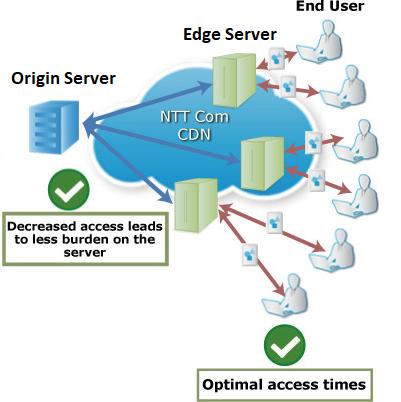
\includegraphics[width=2.2in]{images/cdn.png}

\label{fig:CDN}
\caption{Typical CDN scenario where Origin Server has many Edge Servers to fulfill the Clients requests.}
\end{figure} 

In this scenario, two new trust issues are introduced. First of all, an attacker could modify the content from the Origin Server to the Edge Server. If the indirectly attacked Edge Server serves that modified content, it will be labeled as a misbehaving replica. Secondly, if an Edge Server is not directly managed by the owner of the Origin Server, it can serve different content, such as stale content or outright modified content, adding ads for example.
Furthermore in this architecture the Origin Server is a single point of failure. If the Origin Server is compromised all the Servers misbehave.\\
The main contribute of this work is two-fold.\\First, a new architecture to overcome the trust issue between Servers is suggested, maintaining the CDN properties. Second, it is shown how the system provides a secure method to deliver static content, ensuring the integrity with small effort on Clients and Network. 

\section{Related Works}
Checking the integrity of data retrieved from untrusted Servers is a crucial problem. The typical approach for preventing content tampering between Clients and Servers is to encrypt the end-to-end connection, for example using the SSL protocol.
This negates the functionality of the CDN, because it is always required a connection to the Origin Server, thus the network is no more distributed. For static content, Merkle tree authentication \cite{bayardo2005merkle} is a possible solution, where the Server signs the content which is verified by the Client. Another possible solution are digital rights management schemes, which allow Clients to verify data from an untrusted Server \cite{adelsbach2005towards}. Both these solutions are useless if the Server is compromised. 
For dynamic content, \cite{chi2002xml}\cite{orman2001data} propose the use of XML-based rules for managing the content, but it has to be limited to be easily verified by a Client.\\
In peer-to-peer CDNs these problems are even more significant, because Clients can serve content too. LOCKSS\cite{maniatis2003preserving} uses a voting system for content integrity. 
Repeating the execution to detect misbehavior has been used in Rx\cite{qin2005rx} and in Vigilante \cite{costa2005vigilante} as a method to discover respectively bugs and worms. These approaches imply significant overhead on the Client side. In Pioneer\cite{seshadri2005pioneer} the verify effort is on the dispatcher, a trusted platform, but since the proof of correctness is extremely time sensitive it is not suitable for large scale systems.
Finally the Repeate and Compare system \cite{michalakis2007ensuring}, which is for both static and dynamic content, requires the repetition of the content to another replica and compares the results to detect misbehaving replicas. However, the process has significant overhead, and the verification requests may stress the network, thus only a fraction of the content is verified.\\
In this work Blockchain technology is used. In \cite{kishigami2015blockchain} a video sharing system using a Blockchain is proposed, but implementation details are not provided. The structure of a Blockchain ensures trust between untrusted nodes without a central authority \cite{nakamoto2008bitcoin}. A system of content distribution built on top of a Blockchain inherits all its benefits, making sharing and verifying content between Clients and Servers simple. 


\section{Blockchain Technology}
After the rise of Bitcoin \cite{nakamoto2008bitcoin}, its underlying structure, the Blockchain technology, has been applied to a variety of usecases ranging from authentication \cite{sundararajanonline} (using Ethereum and Smart Contracts) to medical reports\cite{azaria2016medrec}. Blockchain is based on an append-only ledger, a growing list of records (called blocks) which are linked and secured using cryptography. The ledger can be viewed by all participating nodes and the updates are permitted only after the consensum of the network. Each block typically contains a cryptographic hash of the previous block, a timestamp and transaction data. Thanks to its structure and the proof-of-work required to create a new block, a Blockchain is inherently resistant to modification of the data. A simple example of Blockchain is shown in Figure \ref{fig:blockchain}.\\
\begin{figure}[!h]
	\centering
	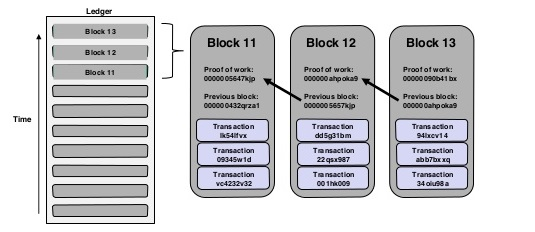
\includegraphics[width=3.8in]{images/blockchain.jpg}
	
	\caption{Example of a Blockchain. Transactions are stored onto the blocks of the Ledger. Blocks are linked by hashes.}
	\label{fig:blockchain}
\end{figure} 

The presented system relies on Ethereum, an open-source, public, Blockchain-based distributed computing platform, which allows the execution of Smart Contracts, immutable programs always visible from the community.


\subsection{Ethereum}
Ethereum \cite{wood2014ethereum} is described as "a transactional singleton machine with shared-state". 
The distributed ledger can be viewed as a distributed virtual machine which records transactions and state changes.
The Blockchain is kept alive by the miners nodes which have three main tasks:
\begin{itemize}
	\item Verifing the transactions being sent, through the consensum algorithm which is similar to other Blockchains, removing the need of central authority;
	\item Checking if the sender has sufficient gas, the Ethereum's native cryptocurrency, to transfer to the receiver;
	\item Running the function called by the sender and thus to modify the Blockchain state accordingly. 
\end{itemize}

In regards to the third point, we see the most important feature of Ethereum: encoding Smart Contracts. 


\subsubsection{Smart Contracts}

Smart Contracts describe functions, which can be called by nodes participating in the Blockchain, and states which can be changed by the nodes. 
The functions run in the Ethereum Virtual Machine (EVM)
which is described as a "\textit{quasi}-Turing complete" computer able to execute code of any complexity. The \textit{quasi} qualification comes from the
fact that the computation is intrinsically bounded to \textit{gas}, which limits the total amount of computation done.
If the gas transferred to the miner for the function execution is less than the required amount, then the transaction is not carried out.  
\\The contract can use memory and storage to save data. It can use any amount of memory (paying gas) during the execution of its code, but when execution ends, the entire content of the memory is wiped. The storage on the other hand is persisted into the Blockchain itself. It can be changed, but all the changes will be recorded onto the ledger.\\
In the presented sytem, thanks to its persistence and (im)mutability, storage will be used to store and share content. 


\subsection{Benefits}
In this paragraph, benefits of using Blockchains are discussed. Since the presented content delivery system is built on top of a Blockchain, it will inherit all its benefits.
\begin{itemize}
	\item \textbf{Decentralization:} a consensus mechanism is used to agree on the validity of transactions, thus there is no need for a trusted third party;
	
	\item \textbf{Transparency and trust:} Blockchains are shared and visible to all the partecipants. This makes the system transparent and as a result trust is established;
	
	\item \textbf{Immutability:} once the data has been written into the Blockchain, it is extremely difficult to change it back. In Ethereum if the state is changed all the updates are stored in the ledger. If only a few users are allowed to change the state, the state will remain immutable as long as they don't change it;
	
	\item \textbf{High availability:} since the system is based on several nodes in a peer-to-peer network, and the data is replicated and updated on each node, the network as a whole continues to work even if nodes leave or become unavailable;
	
	\item \textbf{Highly secure:} all the transactions on a Blockchain are cryptographically secured and provide integrity.
	\vspace{10pt}
\end{itemize} 

\section{System Design}
In this section the developed system to distribute and check integrity of the content is presented. A part of the content is called object, and each object of the content can be verified. Firstly an high-level overview is shown. Secondly more details about the architecture are provided. Lastly benefits and drowbacks of the system are discussed.

\subsection{Overview}
Figure \ref{fig:SystemOverview} shows an high-level view of how the presented system distributes the content on the Servers and permits to Client to check integrity.


\begin{figure}[!h]
	\centering
	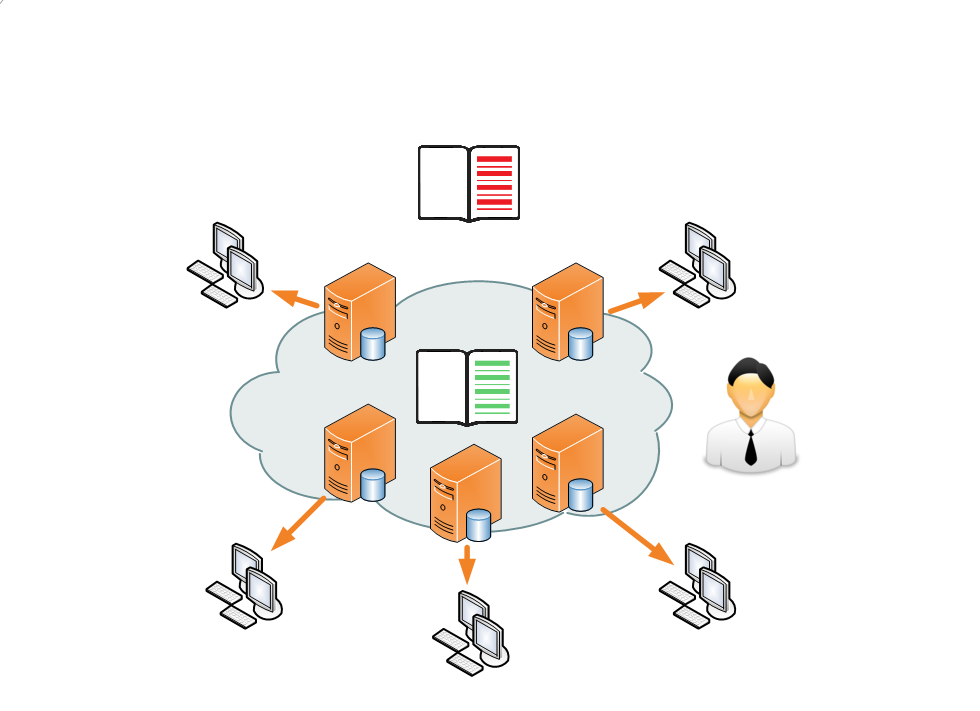
\includegraphics[width=3.8in]{images/SystemOverview.png}
	
	\caption{Overview of the content delivery and check system.}
	\label{fig:SystemOverview}
\end{figure} 

The system wants to resolve trust issues between Origin and Edge Servers, since the latter can receive altered content, and between Servers and Clients, as Servers can send content which differs from the requested one. The key idea is to use two different Blockchains: the \textit{Content Blockchain} and the \textit{Hashes Blockchain}.
\subsubsection{Content Blockchain}
The proposal is to build the CDN on a Blockchain, the \textit{Content Blockchain}. This means that each Edge Server is a node of the Blockchain wherein content will be stored. The Origin Server is no more required, since it is possible to add content from every node (Edge Server) as long as it is authorized, and the content will automatically be distributed on each Server thanks to the Blockchain technology. To authorize the upload of an object of the content an user system is used. Since the Blockchain is always visible to every participant, and every participant has a public address, which consists in a public and private key pair, storing the addresses of who can upload the content in the Blockchain is enough, and after having checked the identity of who is requesting the upload, the transaction can be executed. Two kind of users are permitted: Admin and Superadmin. Admins can upload/remove/edit the content while Superadmins can also create other Admins. 

\subsubsection{Hashes Blockchain}
The \textit{Hashes Blockchain} is the key in checking the integrity of received object of the content. Thanks to hash functions checking message integrity is really simple \cite{tsudik1992message}. An hash function is any function that can be used to map data of arbitrary size to data of fixed size. A cryptographic hash function allows one to easily verify that some input data maps to a given hash value, but if the input data is unknown, it is extremely difficult to reconstruct it by knowing the stored hash value. These property are very useful for the goal. Every time an object of the content is uploaded, its hash is calculated by the Server and stored in the \textit{Hashes Blockchain}, where the partecipants are both Servers and Clients. After the Client receives the requested object it can easily check its integrity calculating its hash and comparing it with the one stored in the Blockchain. If the hashes are equal the object is right, otherwise something wrong happend. Since storing the hash of the object requires the consensum of the network, the hash is always correct, and there is no possibility for a Server to change it without noticing the others nodes. 
	
\subsection{Typical Usage}
A typical use case is shown in Figure \ref{fig:SystemOverview}. First an Admin wants to upload a new content. After the system checks and authorizes him, a new upload request is sent among the \textit{Content Blockchain}. When the network approves the request, a copy of the object is distributed on each Server (according to Blockchain technology) and its hash is calculated and stored in the \textit{Hashes Blockchain}. A Client can ask for that object at any time. When the object is received the Client calculates its hash with the same hash function used by the Server and compares the obtained hash with the calculated one. If they are equal the integrity is verified, otherwise the Client can reject the content and ask to another Server.

\subsection{Benefits and Drawbacks}


In many distributed systems multiple entities maintain their own databases and data sharing can become very difficult due to the disparate nature of the systems. Since a Blockchain can serve as a single shared ledger among interested parties, this can reduce the complexity of managing the whole system, removing the possibile processes of verification, reconciliation, and clearance. The content on all the Servers is always correct and updated, the problem of a replica receiving wrong content from the main Server is avoided.\\
Many of cited systems like Pioneer \cite{seshadri2005pioneer} and Repeat and Compare \cite{michalakis2007ensuring} require sending multiple request to the Server (to get the content and to check it) with the possibility to overcrowd the network, whereas others system causes significant overhead on the Client. In the presented system the traffic needed to check integrity is correlated to the maintaining of the Blockchain itself, which should not be really relevant, and the effort on the Client is minimum as shown in Section \ref{Implementation}. When Client wants to verify the obtained data it just has to calculate an hash, and check the result. Since the checking process is unexpensive for Clients and not stressful for the network, each object of the content can be verified, unlike the other systems where the detection is probabilistic. Furthermore, even the misbehaving Servers detection is simpler thanks to the Blockchain technology. 
\\
Another point of strenght is the removal of the Origin Server; an Admin can simply upload content from his home and it will be distributed among the Servers (peers). Now there is not a single point of failure, since if a Server is compromised the network will know it.  The attacker has to steal the private key of an Admin to take control of a Server, which is difficult, and it is a problem present in any other solution.
\\In this system we have some drawbacks aswell. First of all, all the Servers must have all the content that the system can serve, which can be expensive in some scenarios. However, if the \textit{Content Blockchain} only contained the more requested content or the URIs of the resources, it would be possible to reduces the costs. Secondly, the Clients must have a proxy or some similar mechanism to automatically check the integrity, but this is not a big deal since it can be done with a simple browser add-on for example. Lastly, keeping updated the Blockchain has some costs for the network, but precise tests should be executed to evaluate if this is a real problem, and in a real enviroment the uploading process could be slow due to the mining operation.



\section{Implementation}
\label{Implementation}
The system relies on Ethereum Blockchain and Smart Contracts. Each Smart Contract can have multiple instances. 
The contracts are written in Solidity, a high level language designed to encode contracts in Ethereum. The system was tested on a private Ethereum testnet, which is useful for beginners because the use of money (gas) is not involved. To create the network \textit{geth} was used, the command line interface for running a full ethereum node implemented in Go. The network was composed by few nodes, one Admin and one Superadmin, and a single miner. The difficulty of mining a new block was low, so that testing could be faster.
Different Smart Contracts are developed for \textit{Content Blockchain} and \textit{Hashes Blockchain}. The deploy of contracts was made by Remix IDE, which allows to connect to the private testnet via JSON-RPC. 

\subsection{Content Blockchain}
The \textit{Content Blockchain} is where the content is stored on the Servers. Three Smart Contracts have been written for the scope:
\begin{itemize}
	\item \textbf{StoredContent}: each instance of this contract represents an object of the content. Each object, in addition to data, has the following attributes (stored in the Storage): 
	\begin{itemize}
		\item the owner, that is the uploader Admin;
		\item the name;
		\item the description;
		\item the timestamp of the upload;
		\item the hash.
	\end{itemize}
	Only Admin and Superadmin are allowed to create and manage objects. The contract permits to edit the attributes except the owner, the timestamp and the hash. The last is calculated with \textit{keccak256}, which is an alias of \textit{sha3}. The hash is 32 bytes long;
	\item \textbf{AdminAddresses}: only one instance of this contract is required. It has a map containing the addresses of Admins and Superadmins. Methods to check if an address is related to an Admin and which privileges he has are provided. It is also possible for Superadmins to add or remove Admins using this contract;
	\item \textbf{ContentMap}: only one instance of this contract is required. It has the map of all the objects, wherein the key is the name of the object. Mapped to the key there are the address of the object, its hash, and the names of the other objects related to it (further information are provided in Section \hyperref[sec:Clienthashes]{5.2}). Calling this contract an Admin can add/delete/update any object of the content.
	
\end{itemize}


\subsection{Hashes Blockchain}
\label{sec:Clienthashes}
\begin{figure}[!h]
	\centering
	\includegraphics[width=3.3in]{images/Merkletree.png}
	
	\caption{Example of Merkle Tree. In the root is stored the combination of the hashes stored in the leafs.}
	\label{fig:tree}
\end{figure} 
Assigning to Clients the task of verifying content integrity through hashes would mean that the hash of each object has to be in the \textit{Hashes Blockchain}. Merkle Tree is a perfect data structure for our goals, instead of using a simple Map where each object has its hash. As shown in Figure \ref{fig:tree}, a Merkle Tree is a tree in which every leaf node is labelled with the hash of a data block and every non-leaf node is labelled with the cryptographic hash of the labels of its child nodes. It allows efficient and secure verification of more objects simultaneously. Instead of storing one hash per object, using a Merkle Tree of four leafs, for example, is possible to store one hash every four objects. The number of objects per tree can be increased, with a lot of space saving. In Table \ref{table_space} the required space on Clients using a Map with all the objects versus a Merkle Trees of four objects is shown. 

\begin{table}[!h]
	%% increase table row spacing, adjust to taste
	\renewcommand{\arraystretch}{1.3}
	% if using array.sty, it might be a good idea to tweak the value of
	% \extrarowheight as needed to properly center the text within the cells
	\caption{Example of required space on Clients.}
	\label{table_space}
	\centering
	% Some packages, such as MDW tools, offer better commands for making tables
	%% than the plain LaTeX2e tabular which is used here.
	\begin{tabular}{|c|c|c|}
	\hline
	\textbf{Number of objects} & \textbf{Simple Map} & \textbf{Merkle Tree}\\
	\hline
	\hline
	100'000 & 3,05 Mb & 0,76 Mb\\
	\hline
	1'000'000 & 30,52 Mb & 7,63 Mb \\
	\hline
	30'000'000 & 915,52 Mb & 228,88 Mb\\
	\hline
	\end{tabular}
\end{table}

To check if an object is intact, when the Clients requests that object, the Server sends it with also the hashes of the objects which belong to the same Merkle Tree of the requested object. Then it is sufficient to calculate the root hash of the new Tree composed by the calculated hash of the received object and the hashes of the related objects in the right order, and lastly comparing the result with the root hash stored in the Blockchain. It is almost impossible for the Server to change the content and sending fake hashes for matching the hash stored in the Blockchain, since the hash functions are robust to this attack.\\
Two Smart Contracts have been written for the scope:
\begin{itemize}
	\item \textbf{ObjectsMerkleTree}: each instance of this contract has the root hash of a Merkle Tree. The contract provides methods to calculate, store and check the root hash of four objects;
	\item \textbf{MerkleTreeMap}: only one instance of this contract is required. 
	It maps objects to their Merkle Tree.
\end{itemize}


\section{Future Works}

The presented system has been developed on Ethereum, but it limits the code execution of Smart Contracts imposing gas payment. Some instruction like loops can be very expensive, thus it may not be the best enviroment for the scope. A new ad-hoc Blockchain could be implemented for the content distribution, to better fit the requirments. 
Another improvment could be replacing the data of the content in the \textit{Content Blockchain} with an URI or another type of storage to permit Servers to contain also other objects, depending on the situation.
The idea of using a secure URI would lead to the creation a global Blockchain for content distribution, which different services and websites can entrust with their content. For example, every service can have its own Blockchain, and in the global Blockchain could be links to these Blockchains.
In the end, the presented system is only for static content, a better implementation could be thought for sharing dynamic content too.

% An example of a floating figure using the graphicx package.
% Note that \label must occur AFTER (or within) \caption.
% For figures, \caption should occur after the \includegraphics.
% Note that IEEEtran v1.7 and later has special internal code that
% is designed to preserve the operation of \label within \caption
% even when the captionsoff option is in effect. However, because
% of issues like this, it may be the safest practice to put all your
% \label just after \caption rather than within \caption{}.
%
% Reminder: the "draftcls" or "draftclsnofoot", not "draft", class
% option should be used if it is desired that the figures are to be
% displayed while in draft mode.
%
%\begin{figure}[!t]
%\centering
%\includegraphics[width=2.5in]{myfigure}
% where an .eps filename suffix will be assumed under latex, 
% and a .pdf suffix will be assumed for pdflatex; or what has been declared
% via \DeclareGraphicsExtensions.
%\caption{Simulation results for the network.}
%\label{fig_sim}
%\end{figure}

% Note that the IEEE typically puts floats only at the top, even when this
% results in a large percentage of a column being occupied by floats.


% An example of a double column floating figure using two subfigures.
% (The subfig.sty package must be loaded for this to work.)
% The subfigure \label commands are set within each subfloat command,
% and the \label for the overall figure must come after \caption.
% \hfil is used as a separator to get equal spacing.
% Watch out that the combined width of all the subfigures on a 
% line do not exceed the text width or a line break will occur.
%
%\begin{figure*}[!t]
%\centering
%\subfloat[Case I]{\includegraphics[width=2.5in]{box}%
%\label{fig_first_case}}
%\hfil
%\subfloat[Case II]{\includegraphics[width=2.5in]{box}%
%\label{fig_second_case}}
%\caption{Simulation results for the network.}
%\label{fig_sim}
%\end{figure*}
%
% Note that often IEEE papers with subfigures do not employ subfigure
% captions (using the optional argument to \subfloat[]), but instead will
% reference/describe all of them (a), (b), etc., within the main caption.
% Be aware that for subfig.sty to generate the (a), (b), etc., subfigure
% labels, the optional argument to \subfloat must be present. If a
% subcaption is not desired, just leave its contents blank,
% e.g., \subfloat[].


% An example of a floating table. Note that, for IEEE style tables, the
% \caption command should come BEFORE the table and, given that table
% captions serve much like titles, are usually capitalized except for words
% such as a, an, and, as, at, but, by, for, in, nor, of, on, or, the, to
% and up, which are usually not capitalized unless they are the first or
% last word of the caption. Table text will default to \footnotesize as
% the IEEE normally uses this smaller font for tables.
% The \label must come after \caption as always.
%
%\begin{table}[!t]
%% increase table row spacing, adjust to taste
%\renewcommand{\arraystretch}{1.3}
% if using array.sty, it might be a good idea to tweak the value of
% \extrarowheight as needed to properly center the text within the cells
%\caption{An Example of a Table}
%\label{table_example}
%\centering
%% Some packages, such as MDW tools, offer better commands for making tables
%% than the plain LaTeX2e tabular which is used here.
%\begin{tabular}{|c||c|}
%\hline
%One & Two\\
%\hline
%Three & Four\\
%\hline
%\end{tabular}
%\end{table}


% Note that the IEEE does not put floats in the very first column
% - or typically anywhere on the first page for that matter. Also,
% in-text middle ("here") positioning is typically not used, but it
% is allowed and encouraged for Computer Society conferences (but
% not Computer Society journals). Most IEEE journals/conferences use
% top floats exclusively. 
% Note that, LaTeX2e, unlike IEEE journals/conferences, places
% footnotes above bottom floats. This can be corrected via the
% \fnbelowfloat command of the stfloats package.




\section{Conclusion}

In the presented system a solution is found for trust issues in a Content Distribution Network. Thanks to the growing Blockchain technology and its security characteristics, it is possible to securely distribute content among Servers, and a Client can check if the requested content is intact. Many problems of exiting systems like strong efforts on the Network or Clients are solved, and the prototype built on the private Ethereum testnet shows the feasibilty of such system. The use of Merkle Tree leads to space saving, and with other smaller improvements the bootstrap of the system should be a real possibility.





% trigger a \newpage just before the given reference
% number - used to balance the columns on the last page
% adjust value as needed - may need to be readjusted if
% the document is modified later
%\IEEEtriggeratref{8}
% The "triggered" command can be changed if desired:
%\IEEEtriggercmd{\enlargethispage{-5in}}

% references section

% can use a bibliography generated by BibTeX as a .bbl file
% BibTeX documentation can be easily obtained at:
% http://mirror.ctan.org/biblio/bibtex/contrib/doc/
% The IEEEtran BibTeX style support page is at:
% http://www.michaelshell.org/tex/ieeetran/bibtex/
\bibliographystyle{IEEEtran}
% argument is your BibTeX string definitions and bibliography database(s)
\bibliography{references}
%
% <OR> manually copy in the resultant .bbl file
% set second argument of \begin to the number of references
% (used to reserve space for the reference number labels box)

%\begin{thebibliography}{1}

%\bibitem{IEEEhowto:kopka}
%H.~Kopka and P.~W. Daly, \emph{A Guide to \LaTeX}, 3rd~ed.\hskip 1em plus
%  0.5em minus 0.4em\relax Harlow, England: Addison-Wesley, 1999.

%\end{thebibliography}




% that's all folks
\end{document}


